%% The openany option is here just to remove the blank pages before a new chapter
\documentclass[11pt,openany]{book}

\title{Endnotes using pagenote package at the end of a book}

\usepackage{pagenote}

%%%%%%%%%%%%% For customising the endnote markers. Comment these out if you don't want them.
% To prefix each note number with the chapter number
\renewcommand{\thepagenote}{\thechapter-\arabic{pagenote}}

% To have a slightly different formatting for the endnote numbers in the text -- smaller text, sans-serif, square brackets
\renewcommand\notenumintext[1]{\space{\footnotesize\sffamily[FN-#1]}}

% To have a slightly different formatting for the endnote numbers in the notes section. Just the square brackets and sans-serif; normal size.
\renewcommand\notenuminnotes[1]{{\sffamily[FN-#1] }}

% If you want a different name/heading for the end notes
\renewcommand{\notesname}{End Notes}
%%%%%%%%%%%%% End customisation


%% THIS LINE IS MANDATORY
\makepagenote

\usepackage{hyperref}
\usepackage{minted}
\usepackage{graphicx}

\graphicspath{img/}

\begin{document}

\chapter{TensorFlow}
\section{Intruduction}
TensorFlow is a framework for numerical computation using data flow graphs. Nodes in the graph represent mathematical operations, and the graph edges represent the multidimensional data arrays (tensors) communicated between them. This architecture gives flexibility as process some nodes on a GPU and others on a CPU, or process the graph in a cluster.

For example, if we want sum two constants using TensorFlow:

\begin{minted}{python}
node1 = tf.constant(3.0, dtype=tf.float32)
node2 = tf.constant(4.0)
node3 = tf.add(node1, node2)

sess = tf.Session()
print(sess.run(node3))
\end{minted}

This piece of code gives 7.0 as a result, so how it works, first we assembly the graph, after we create a session and run this graph to get a result, the runtime is outside Python, in fact all back-end of TensorFlow is wrote in C++, and can use GPU to accelerate the process, so to avoid any copy from CPU to GPU what is slow, all graph must me assembled before to be executed.

\section{Nodes and operations}
The piece of cod above gives the follow graph:

\begin{figure}[h]
    \centering
    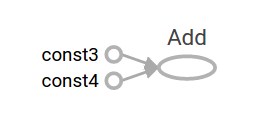
\includegraphics[width=0.8\textwidth]{img/const_add.png}
    \caption{nodes of constants sum graph}
    \label{fig:const_add}
\end{figure}

Sum constants is not so useful, so TensorFlow has others kind of input nodes, as variables and placeholders, and a node can make an operation as sum, multiplication, convolution and others.

\section{The model}

The TensorFlow model is the graph nodes and the weights, and all of TensorFlow's file formats are based on Protocol Buffers.

\subsection{graph}
The main object of TensorFlow is the graph, this holds a network of nodes, each representing one operation, connected to each other as inputs and outputs.

\begin{minted}{protobuf}
message GraphDef {
  repeated NodeDef node = 1;
  int32 version = 3 [deprecated = true];
  FunctionDefLibrary library = 2;
};
\end{minted}

Where the keyword repeated say to protobuf that GraphDef has several instance of NodeDef, in fact it is the heart of TensorFlow's model.

\subsection{Nodes}

The NodeDef object  are the fundamental building blocks of TensorFlow graphs, with each one defining a single operation along with its input connections. Here are the protobuf definition of NodeDef.

\begin{minted}{protobuf}
message NodeDef {
  string name = 1;
  string op = 2;
  repeated string input = 3;
  string device = 4;
  map<string, AttrValue> attr = 5;
};
\end{minted}

\subsubsection{name}
Every node should have a unique identifier that's not used by any other nodes in the graph. The name is used when defining the connections between nodes, and when setting inputs and outputs for the whole graph when it's run.

\subsubsection{op}
This defines what operation to run, for example "Add", "MatMul", or "Conv2D".

\subsubsection{input}
A list of strings, each one of which is the name of another node. For example, a node with two inputs might have a list like \["some_node_name", "another_node_name"\].

\subsubsection{device}
Defines where to run a node in a distributed environment, or when you want to force the operation onto CPU or GPU.

\subsubsection{attr}
This is a key/value store holding all the attributes of a node. These are the permanent properties of nodes, it means, they don't change when you run the graph, for example, a constant value can't change when you run the graph.
Each attribute has a unique name string, and the expected attributes are listed when the operation is defined. If an attribute isn't present in a node, but it has a default listed in the operation definition, that default is used when the graph is created.

The protobuf definition for attr.

\begin{minted}{protobuf}
import "tensorflow/core/framework/tensor.proto";
import "tensorflow/core/framework/tensor_shape.proto";
import "tensorflow/core/framework/types.proto";

message AttrValue {
  message ListValue {
    repeated bytes s = 2;                        // "list(string)"
    repeated int64 i = 3 [packed = true];        // "list(int)"
    repeated float f = 4 [packed = true];        // "list(float)"
    repeated bool b = 5 [packed = true];         // "list(bool)"
    repeated DataType type = 6 [packed = true];  // "list(type)"
    repeated TensorShapeProto shape = 7;         // "list(shape)"
    repeated TensorProto tensor = 8;             // "list(tensor)"
    repeated NameAttrList func = 9;              // "list(attr)"
  }

  oneof value {
    bytes s = 2;                 // "string"
    int64 i = 3;                 // "int"
    float f = 4;                 // "float"
    bool b = 5;                  // "bool"
    DataType type = 6;           // "type"
    TensorShapeProto shape = 7;  // "shape"
    TensorProto tensor = 8;      // "tensor"
    ListValue list = 1;          // any "list(...)"

    NameAttrList func = 10;

    string placeholder = 9;
  }
}

message NameAttrList {
  string name = 1;
  map<string, AttrValue> attr = 2;
}
\end{minted}

\subsection{Weights}

The main use of TensorFlow today is to create, train and run neural network, so we need a way to store this waits in the model. A common way to store them, for example in graphs created by the freeze\_graph script, is as Const ops containing the weights as Tensors. These are defined in protobuf.

\begin{minted}{protobuf}
message TensorProto {
  TensorShapeProto tensor_shape = 2;
  int32 version_number = 3;
  bytes tensor_content = 4;
  repeated int32 half_val = 13 [packed = true];
  repeated float float_val = 5 [packed = true];
  repeated double double_val = 6 [packed = true];
  repeated int32 int_val = 7 [packed = true];
  repeated bytes string_val = 8;
  repeated float scomplex_val = 9 [packed = true];
  repeated int64 int64_val = 10 [packed = true];
  repeated bool bool_val = 11 [packed = true];
  repeated double dcomplex_val = 12 [packed = true];
  repeated ResourceHandleProto resource_handle_val = 14;
  repeated VariantTensorDataProto variant_val = 15;
};

message VariantTensorDataProto {
  string type_name = 1;
  bytes metadata = 2;
  repeated TensorProto tensors = 3;
}
\end{minted}

The Tensor object can be stored in a constant node for example.

\chapter{XLA}

XLA (Accelerated Linear Algebra) is a compiler for linear algebra that optimizes TensorFlow computations. XLA works with just-in-time (JIT) compilation or ahead-of-time (AOT) compilation, and the objectives are Improve execution speed, Improve memory usage, Reduce reliance on custom Ops , Reduce mobile footprint and Improve portability.

The input language to XLA is called "HLO IR", or just HLO (High Level Optimizer), the HLO can be understood like LLVM IR.

The following diagram shows the compilation process in XLA:

\begin{figure}[h]
    \centering
    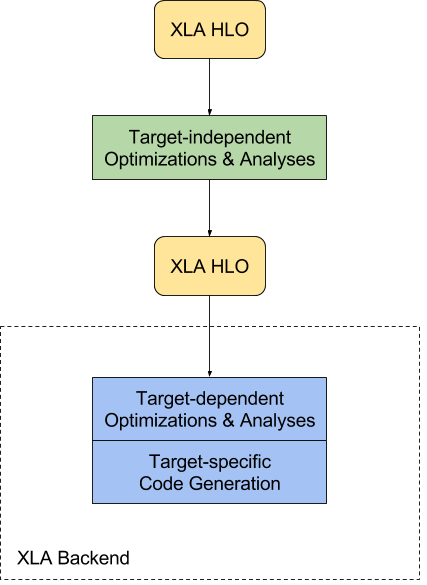
\includegraphics[width=0.8\textwidth]{img/how-does-xla-work.png}
    \caption{compilation process in XLA}
    \label{fig:const_add}
\end{figure}

The target-specific code generation. The CPU and GPU back-ends included with XLA use LLVM for low-level IR, optimization, and code-generation. These back-ends emit the LLVM IR necessary to represent the XLA HLO computation in an efficient manner, and then invoke LLVM to emit native code from this LLVM IR.

So, if we want that XLA support a new architecture we only have to change the last layer, and it is possible add new architectures extending some classes.

\section{Developing a new back-end for XLA}

XLA provides an abstract interface that a new architecture or accelerator can implement to create a backend to run TensorFlow graphs. It is need knowledge of LLVM, Bazel, and TensorFlow.

\section{JIT Compilation}

\section{AOT compilation}
\subsection{tfcompile}

tfcompile is a standalone tool that ahead-of-time (AOT) compiles TensorFlow graphs into executable code. 





\appendix %% Up to you -- I just like to have the end notes as an appendix :-)
\printnotes*

\end{document}